%File: anonymous-submission-latex-2026.tex
\documentclass[letterpaper]{article} % DO NOT CHANGE THIS
\usepackage[submission]{aaai2026}  % DO NOT CHANGE THIS
\usepackage{times}  % DO NOT CHANGE THIS
\usepackage{helvet}  % DO NOT CHANGE THIS
\usepackage{courier}  % DO NOT CHANGE THIS
\usepackage[hyphens]{url}  % DO NOT CHANGE THIS
\usepackage{graphicx} % DO NOT CHANGE THIS
\usepackage{amsmath}  % For mathematical typesetting
\urlstyle{rm} % DO NOT CHANGE THIS
\def\UrlFont{\rm}  % DO NOT CHANGE THIS
\usepackage{natbib}  % DO NOT CHANGE THIS AND DO NOT ADD ANY OPTIONS TO IT
\usepackage{caption} % DO NOT CHANGE THIS AND DO NOT ADD ANY OPTIONS TO IT
\frenchspacing  % DO NOT CHANGE THIS
\setlength{\pdfpagewidth}{8.5in} % DO NOT CHANGE THIS
\setlength{\pdfpageheight}{11in} % DO NOT CHANGE THIS
%
% These are recommended to typeset algorithms but not required. See the subsubsection on algorithms. Remove them if you don't have algorithms in your paper.
\usepackage{algorithm}
\usepackage{algorithmic}

%
% These are are recommended to typeset listings but not required. See the subsubsection on listing. Remove this block if you don't have listings in your paper.
\usepackage{newfloat}
\usepackage{listings}
\DeclareCaptionStyle{ruled}{labelfont=normalfont,labelsep=colon,strut=off} % DO NOT CHANGE THIS
\lstset{%
	basicstyle={\footnotesize\ttfamily},% footnotesize acceptable for monospace
	numbers=left,numberstyle=\footnotesize,xleftmargin=2em,% show line numbers, remove this entire line if you don't want the numbers.
	aboveskip=0pt,belowskip=0pt,%
	showstringspaces=false,tabsize=2,breaklines=true}
\floatstyle{ruled}
\newfloat{listing}{tb}{lst}{}
\floatname{listing}{Listing}
%
% Keep the \pdfinfo as shown here. There's no need
% for you to add the /Title and /Author tags.
\pdfinfo{
/TemplateVersion (2026.1)
}

% DISALLOWED PACKAGES
% \usepackage{authblk} -- This package is specifically forbidden
% \usepackage{balance} -- This package is specifically forbidden
% \usepackage{color (if used in text)
% \usepackage{CJK} -- This package is specifically forbidden
% \usepackage{float} -- This package is specifically forbidden
% \usepackage{flushend} -- This package is specifically forbidden
% \usepackage{fontenc} -- This package is specifically forbidden
% \usepackage{fullpage} -- This package is specifically forbidden
% \usepackage{geometry} -- This package is specifically forbidden
% \usepackage{grffile} -- This package is specifically forbidden
% \usepackage{hyperref} -- This package is specifically forbidden
% \usepackage{navigator} -- This package is specifically forbidden
% (or any other package that embeds links such as navigator or hyperref)
% \indentfirst} -- This package is specifically forbidden
% \layout} -- This package is specifically forbidden
% \multicol} -- This package is specifically forbidden
% \nameref} -- This package is specifically forbidden
% \usepackage{savetrees} -- This package is specifically forbidden
% \usepackage{setspace} -- This package is specifically forbidden
% \usepackage{stfloats} -- This package is specifically forbidden
% \usepackage{tabu} -- This package is specifically forbidden
% \usepackage{titlesec} -- This package is specifically forbidden
% \usepackage{tocbibind} -- This package is specifically forbidden
% \usepackage{ulem} -- This package is specifically forbidden
% \usepackage{wrapfig} -- This package is specifically forbidden
% DISALLOWED COMMANDS
% \nocopyright -- Your paper will not be published if you use this command
% \addtolength -- This command may not be used
% \balance -- This command may not be used
% \baselinestretch -- Your paper will not be published if you use this command
% \clearpage -- No page breaks of any kind may be used for the final version of your paper
% \columnsep -- This command may not be used
% \newpage -- No page breaks of any kind may be used for the final version of your paper
% \pagebreak -- No page breaks of any kind may be used for the final version of your paperr
% \pagestyle -- This command may not be used
% \tiny -- This is not an acceptable font size.
% \vspace{- -- No negative value may be used in proximity of a caption, figure, table, section, subsection, subsubsection, or reference
% \vskip{- -- No negative value may be used to alter spacing above or below a caption, figure, table, section, subsection, subsubsection, or reference

\setcounter{secnumdepth}{0} %May be changed to 1 or 2 if section numbers are desired.

% The file aaai2026.sty is the style file for AAAI Press
% proceedings, working notes, and technical reports.
%

% Title

% Your title must be in mixed case, not sentence case.
% That means all verbs (including short verbs like be, is, using,and go),
% nouns, adverbs, adjectives should be capitalized, including both words in hyphenated terms, while
% articles, conjunctions, and prepositions are lower case unless they
% directly follow a colon or long dash
\title{Video Comprehension Score (VCS): A Metric for Long-Form Video Description Evaluation}
\author{
    %Authors
    % All authors must be in the same font size and format.
    Written by AAAI Press Staff\textsuperscript{\rm 1}\thanks{With help from the AAAI Publications Committee.}\\
    AAAI Style Contributions by Pater Patel Schneider,
    Sunil Issar,\\
    J. Scott Penberthy,
    George Ferguson,
    Hans Guesgen,
    Francisco Cruz\equalcontrib,
    Marc Pujol-Gonzalez\equalcontrib
}
\affiliations{
    %Afiliations
    \textsuperscript{\rm 1}Association for the Advancement of Artificial Intelligence\\
    % If you have multiple authors and multiple affiliations
    % use superscripts in text and roman font to identify them.
    % For example,

    % Sunil Issar\textsuperscript{\rm 2},
    % J. Scott Penberthy\textsuperscript{\rm 3},
    % George Ferguson\textsuperscript{\rm 4},
    % Hans Guesgen\textsuperscript{\rm 5}
    % Note that the comma should be placed after the superscript

    1101 Pennsylvania Ave, NW Suite 300\\
    Washington, DC 20004 USA\\
    % email address must be in roman text type, not monospace or sans serif
    proceedings-questions@aaai.org
%
% See more examples next
}

%Example, Single Author, ->> remove \iffalse,\fi and place them surrounding AAAI title to use it
\iffalse
\title{My Publication Title --- Single Author}
\author {
    Author Name
}
\affiliations{
    Affiliation\\
    Affiliation Line 2\\
    name@example.com
}
\fi

\iffalse
%Example, Multiple Authors, ->> remove \iffalse,\fi and place them surrounding AAAI title to use it
\title{My Publication Title --- Multiple Authors}
\author {
    % Authors
    First Author Name\textsuperscript{\rm 1},
    Second Author Name\textsuperscript{\rm 2},
    Third Author Name\textsuperscript{\rm 1}
}
\affiliations {
    % Affiliations
    \textsuperscript{\rm 1}Affiliation 1\\
    \textsuperscript{\rm 2}Affiliation 2\\
    firstAuthor@affiliation1.com, secondAuthor@affilation2.com, thirdAuthor@affiliation1.com
}
\fi


% REMOVE THIS: bibentry
% This is only needed to show inline citations in the guidelines document. You should not need it and can safely delete it.
\usepackage{bibentry}
% END REMOVE bibentry

\begin{document}

\maketitle

\begin{figure*}[t]
\centering
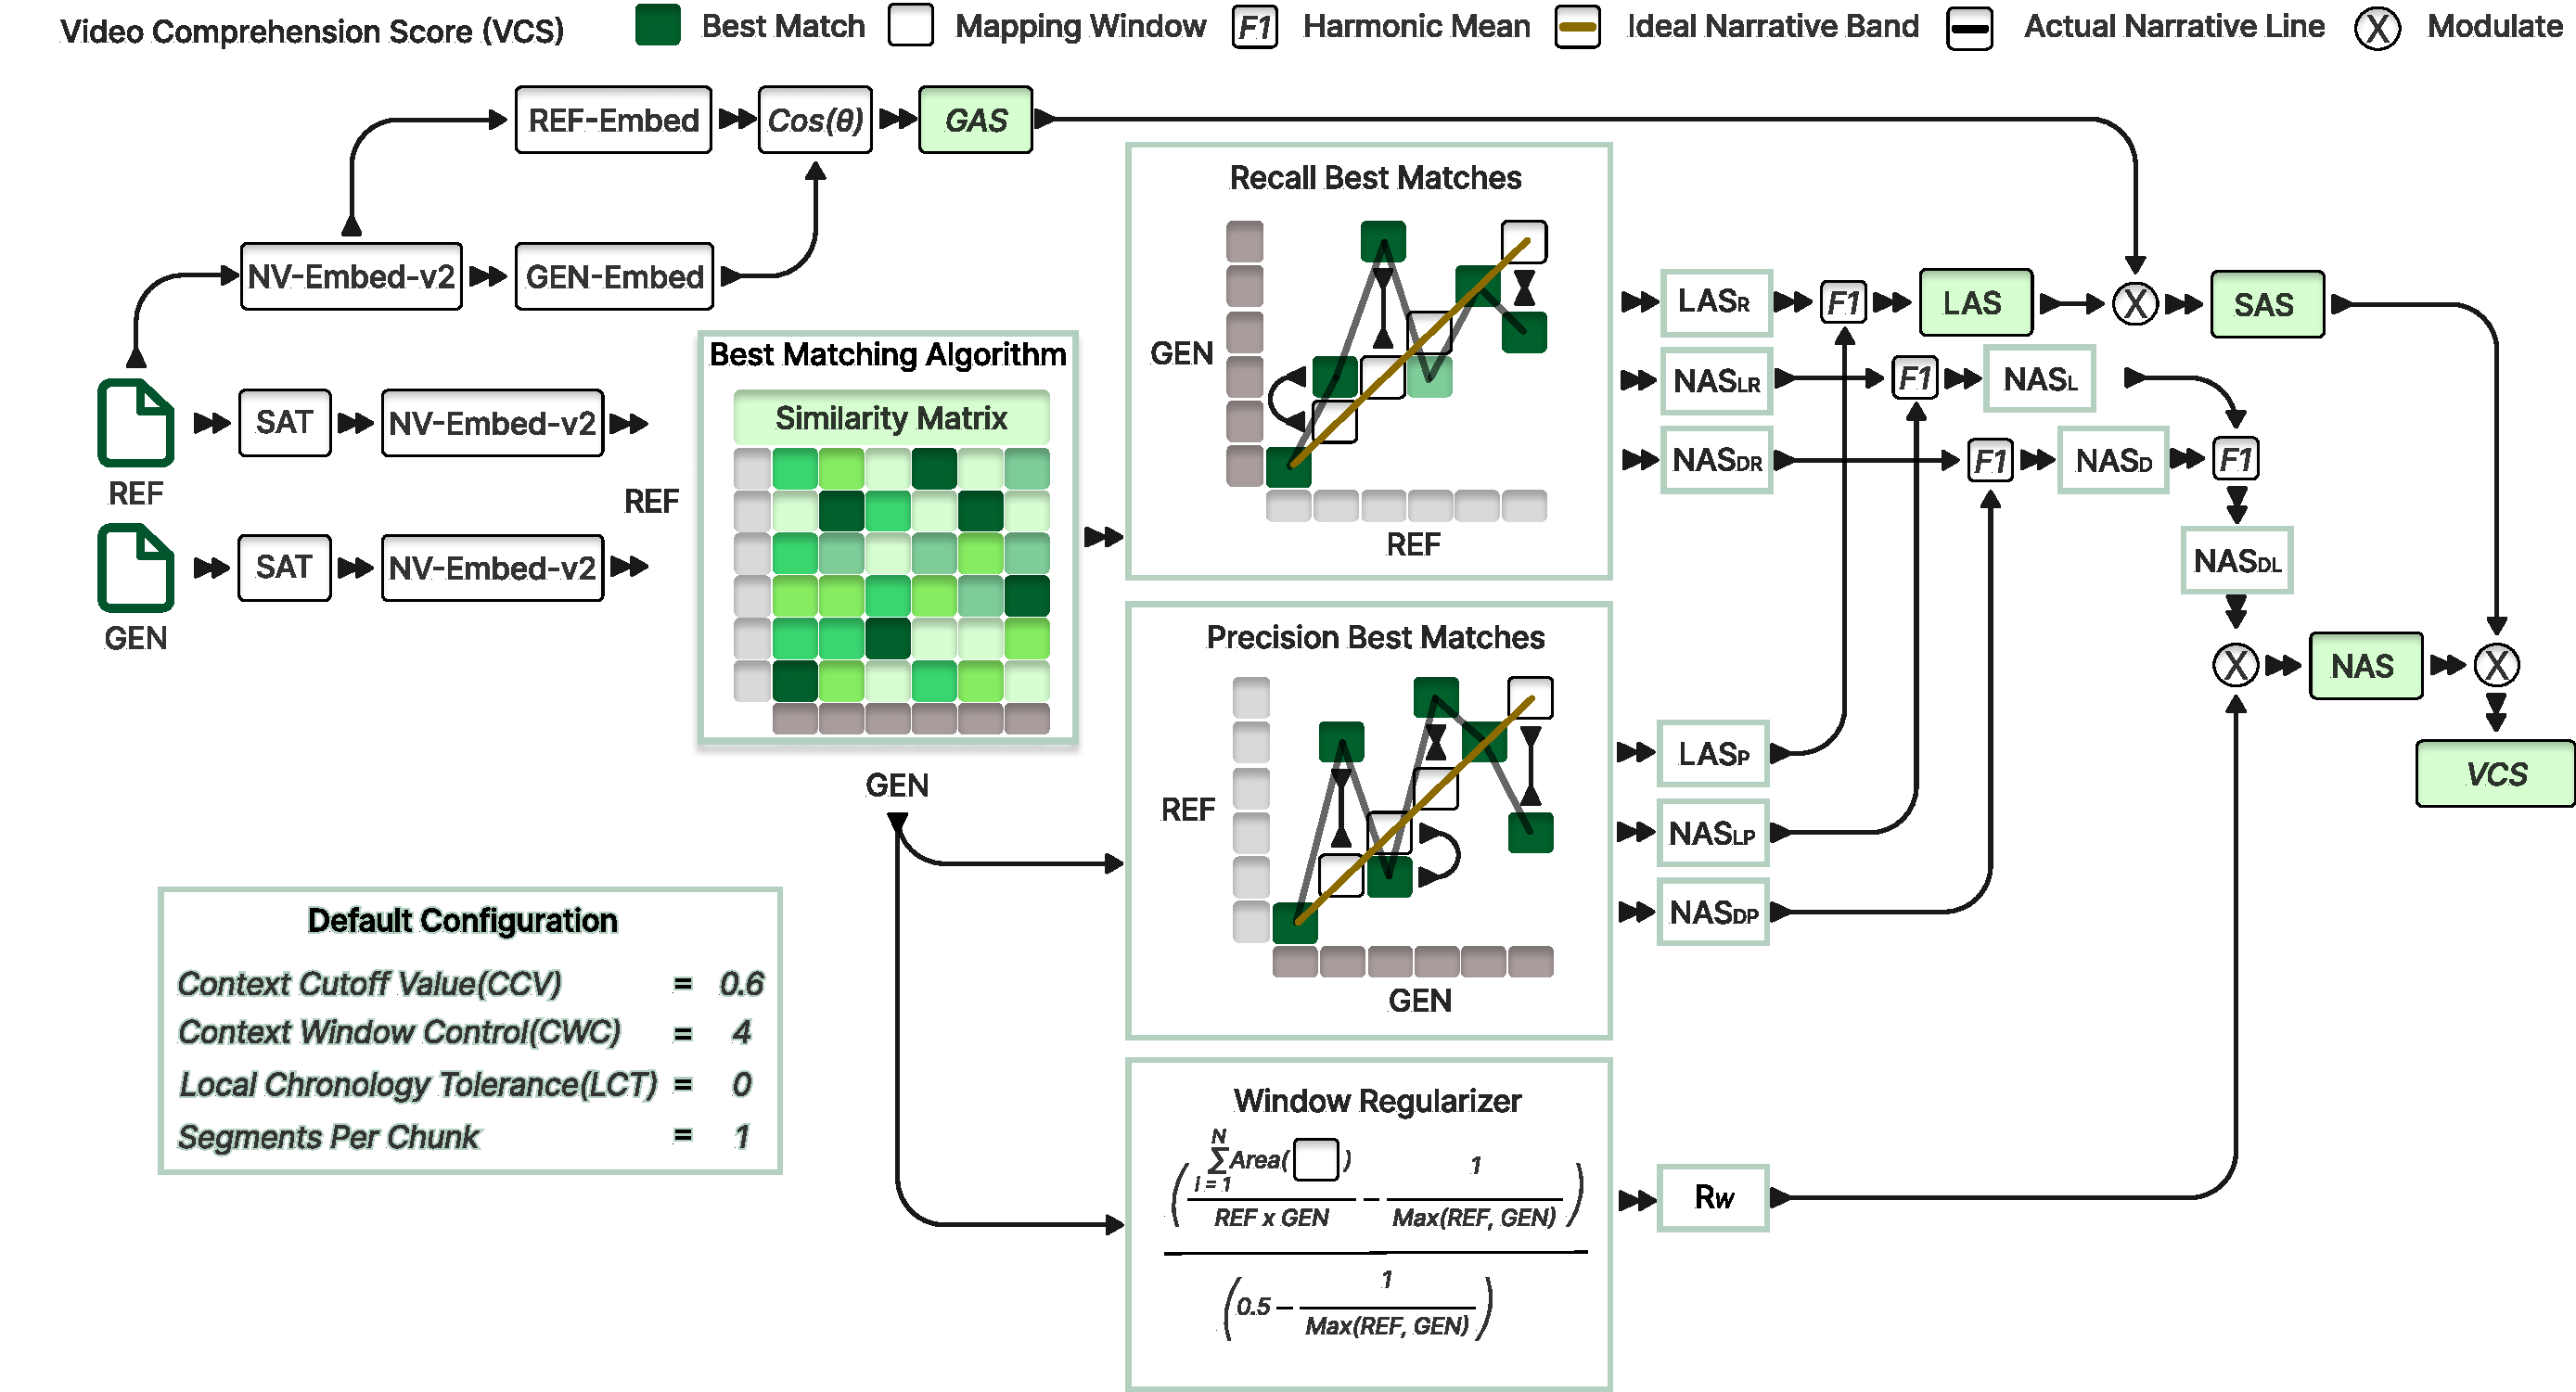
\includegraphics[width=0.8\textwidth]{VCS}
\caption{Architecture of the Video Comprehension Score (VCS). The VCS assesses video descriptions by comparing a reference text ($T_{ref}$) with a model-generated text ($T_{gen}$). Both texts are initially segmented by SaT and embedded via nvEmbed. The Global Alignment Score (GAS) is computed from the full text embeddings. For localized analysis, texts are chunked and embedded, forming a similarity matrix. From this, precision and recall-oriented best matches yield the Local Alignment Score (LAS)—the harmonic mean of $LAS_P$ (precision) and $LAS_R$ (recall). The Narrative Alignment Score (NAS) incorporates distance-based ($NAS_D$) and line-based ($NAS_L$) assessments. $NAS_D$ and $NAS_L$ are harmonic means of their respective precision and recall components. A Window Regularizer ($R_w$) refines the NAS. The Semantic Alignment Score (SAS) is derived by modulating GAS with LAS. The final VCS results from modulating the smaller of SAS and the regularized NAS with the larger.}
\label{fig:vcs-architecture}
\end{figure*}

\begin{abstract}
Evaluating long-form video descriptions is challenging, as traditional metrics like BLEU, ROUGE, and METEOR inadequately capture narrative coherence, temporal ordering, and semantic equivalence beyond lexical overlap. We introduce Video Comprehension Score (VCS), a comprehensive metric assessing semantic alignment, temporal accuracy, and corruption sensitivity. VCS integrates three components: Global Alignment Score for global thematic similarity, Local Alignment Score for local semantic correspondence, and Narrative Alignment Score for temporal coherence with adjustable tolerance. VCS is validated on two large-scale synthetic test sets derived from 1,390 scene-level descriptions from the MPII Movie Description dataset. For the Comparison Test Set, these scenes are aggregated into baseline descriptions ($\approx$500 words each) via ChatGPT-4o, then augmented with 10 valid and 10 invalid stylistic or corrupt variants, totaling 27,800 descriptions. For the Multiple-Author Test Set, the same 1,390 scene-level descriptions are aggregated using four different LLMs, resulting in 5,560 descriptions representing realistic authorial variation. VCS consistently outperforms traditional metrics, being the only metric capable of distinguishing valid from invalid variants in the Comparison Test Set. On the Multiple-Author Test Set, it achieves superior cross-author consistency, being the only metric with $>$80\% accuracy across four language model references. VCS$_{\text{short}}$, our implementation of VCS for short captions, attains state-of-the-art human correlation on VATEX-EVAL in the 9-ref setting (Kendall's $\tau=41.5$, Spearman's $\rho=52.8$) and competitive results in the 1-ref setting (Kendall's $\tau=30.0$, Spearman's $\rho=38.1$). These results demonstrate the effectiveness of VCS for robustly assessing video description quality across diverse narrative styles and lengths.
\end{abstract}

% Uncomment the following to link to your code, datasets, an extended version or similar.
% You must keep this block between (not within) the abstract and the main body of the paper.
% \begin{links}
%     \link{Code}{https://aaai.org/example/code}
%     \link{Datasets}{https://aaai.org/example/datasets}
%     \link{Extended version}{https://aaai.org/example/extended-version}
% \end{links}

\section{Introduction}

Recent advancements in Large Video Language Models (LVLMs) \citep{Yuan2025Tarsier2,Shen2025LongVU,Ataallah2024Goldfish,Chen2025LongVILA} have substantially enhanced automated video comprehension, enabling extensive and detailed descriptions from complex content. This advancement is critical for applications requiring nuanced interpretation, such as autonomous navigation and assistive technologies. However, accurately evaluating genuine comprehension—rather than frame-level element identification—remains challenging, particularly with long videos. Existing evaluation frameworks primarily utilize question-answering or caption-based methods \citep{wu2024longvideobench,ataallah2024infinibench,mangalam2023egoschema,zhou2025mlvu}. Question-answering effectively probes specific details but inadequately measures holistic comprehension. Caption-based methods better capture overall narrative comprehension but fail to effectively assess specific detail recognition. Given our primary concern with comprehensive video comprehension, caption-based evaluations are more suitable.

Traditional caption-based evaluation techniques include n-gram metrics such as BLEU \citep{p:02}, METEOR \citep{bl:05}, CIDEr \citep{v:15}, and ROUGE \citep{l:04}, embedding-based metrics such as BERTScore \citep{z:20}, and contemporary LLM-based approaches such as CLAIR \citep{chan:23} and AutoDQ \citep{wyzs:24}, each exhibiting critical shortcomings with extensive LVLM-generated descriptions. N-gram metrics rely on lexical overlap, unfairly penalizing legitimate stylistic variations, increasingly problematic as description length grows. Embedding-based metrics address lexical overlap by focusing on semantic similarity but remain constrained by limited context lengths, less effective for very long descriptions, and inadequately evaluate chronological accuracy. LLM-driven methods provide deeper semantic insights but depend heavily on the inherent accuracy of the underlying LLM and often lack consistency.

Evaluating long-form descriptions introduces two principal challenges:
\begin{enumerate}
\item \textbf{Expressive Variability}: Extended descriptions allow multiple valid articulations differing in detail, style, and length. Conversely, invalid expressions involving omissions or distortions may occur. An effective evaluation metric must discriminate valid variations without unnecessary penalties and detect invalid articulations accurately.
\item \textbf{Narrative Variability}: Extended descriptions may validly represent events in different chronological sequences or present genuinely incorrect sequences. A robust evaluation method must distinguish valid variations without unjust penalties while identifying incorrect sequences accurately.
\end{enumerate}

This paper introduces the Video Comprehension Score (VCS), a novel metric addressing these complexities by evaluating dense, long-form descriptions semantically and structurally. VCS employs Segment Any Text (SaT) \citep{frohmann-etal-2024-segment} for semantic segmentation and NvEmbed-v2 \citep{l:24} for paragraph and chunk-level embeddings, comprising three components:
\begin{enumerate}
\item \textbf{Global Alignment Score (GAS)}: Measures overall thematic similarity using full-text embeddings.
\item \textbf{Local Alignment Score (LAS)}: Assesses fine-grained semantic correspondence between chunks.
\item \textbf{Narrative Alignment Score (NAS)}: Evaluates chronological consistency using a configurable local chronology tolerance factor (LCT) to control the strictness of chronological evaluation.
\end{enumerate}

Combining GAS and LAS yields the Semantic Alignment Score (SAS), representing semantic alignment across long paragraphs. Integrating SAS with NAS produces the comprehensive VCS metric, clearly assessing narrative equivalence between model-generated and human-written descriptions. Additionally, we generalize VCS to VCS$_{\text{short}}$, applying the same principles to shorter captions.

Due to the absence of suitable annotated datasets for dense, long-form descriptions—where human judgment becomes increasingly unreliable—we constructed a large-scale synthetic dataset (1390 descriptions, $\sim$500 words each, from the MPII Movie Description dataset \citep{rohrbach2015dataset} via ChatGPT4o). Two test sets, a Comparison Test Set (27,800 description pairs) and a Multiple-Author Test Set (5560 variants from four LLMs), comprehensively evaluate VCS performance. Benchmarked against traditional metrics (BLEU, METEOR, ROUGE and etc.), VCS consistently demonstrated insensitivity to valid variations and sensitivity to invalid variations as compared to traditional metrics. On VATEX-EVAL, VCS$_{\text{short}}$ achieved state-of-the-art results in the 9-reference setting and a close second in the 1-reference setting. Results affirm VCS as a reliable metric accurately assessing narrative equivalence across diverse descriptive styles and lengths, configurable for varying chronological rigor.

Our primary contributions include:
\begin{itemize}
\item A robust metric (VCS) for both long-form and short-form video descriptions.
\item Configurable LCT and chunk size parameters to govern chronological strictness and comparison granularity.
\end{itemize}

\section{Related Work}

Traditional n-gram-based metrics such as BLEU \citep{p:02}, ROUGE \citep{l:04}, and METEOR \citep{bl:05} evaluate text generation through lexical overlap and local word order. BLEU measures n-gram precision with brevity penalties, capturing local chronology but struggles with expressive variability. ROUGE variants emphasize recall; ROUGE-N evaluates n-gram overlap, while ROUGE-L utilizes the Longest Common Subsequence (LCS) at sentence-level, yet remains sensitive to expressive variability and sentence-length discrepancies. METEOR addresses expressive variability via synonyms and stems, computing precision-recall harmonics with fragmentation penalties for local word order. CIDEr \citep{v:15} addresses expressive variability by consensus-based TF-IDF weighting across multiple references but proves impractical for long-form descriptions due to labor-intensive annotation. SPICE \citep{afjg:16} evaluates semantic propositions using graph overlaps, effectively handling paraphrasing; however, being designed for static images, it cannot be directly applied to videos and neglects the fluency, grammar, and narrative chronology critical for video descriptions.

Embedding-based metrics compare texts in semantic vector spaces, leveraging pretrained models to capture semantic similarity beyond lexical matches. Early methods like BERTScore \citep{z:20}, MoverScore \citep{z:19}, and SBERT \citep{r:19} address expressive variability by recognizing paraphrases but are constrained by limited context windows, complicating their direct application to long-form descriptions. Recent decoder-based models such as nv-embed-v2 \citep{l:24}, Linq-Embed-Mistral \citep{cklg:24}, SFR-Embedding-Mistral \citep{mljx:24}, and Jasper and Stella \citep{zlw:24} offer significantly larger context windows and robust global embeddings, excelling at paragraph-level semantic assessments. However, reliance on global embeddings and cosine similarity overlooks local content alignment, detailed information accuracy, and chronological coherence, allowing subtle inaccuracies or misordered events to remain undetected.

Multimodal embedding metrics like EMScore \citep{syxl:22} and PAC-S \citep{sbc:23} employ vision-language models such as CLIP \citep{Radford2021LearningTV} to evaluate semantic alignment between visuals and generated captions, addressing expressive variability through direct image-caption comparison, thus bypassing reference caption. EMScore combines coarse and fine-grained multimodal matches for accurate short-caption evaluation, whereas PAC-S, fine-tuned via contrastive learning, closely aligns with human judgments. Despite their effectiveness in short-form descriptions, these metrics face computational challenges and methodological limitations when scaling to long-form descriptions.

Recent evaluation approaches increasingly leverage Large Language Models (LLMs), categorized into component-based and holistic judge methods. Component-based methods such as AutoDQ \citep{wyzs:24} and VAD-Score \citep{dp:25} use LLMs for semantic extraction and entailment checks, effectively addressing the expressive variability challenge; however, AutoDQ and VAD do not evaluate the chronology of events. Nonetheless, their effectiveness depends heavily on extraction accuracy, consistency across model updates, scalability with dense content, and reliance on comprehensive references. Conversely, holistic methods such as CapScore \citep{li:24}, CapArena‑Auto Score \citep{cheng:25}, and CLAIR \citep{chan:23} provide overall quality assessments directly from LLMs, theoretically addressing complex evaluation dimensions comprehensively. However, they suffer from ambiguity in score calibration, sensitivity to prompting nuances, consistency issues across model versions, limited interpretability, and practical constraints, including reproducibility and cost.

\section{Methodology: Video Comprehension Score (VCS)}
\label{sec:methodology_vcs}

Figure~\ref{fig:VCS} illustrates the overall architecture of the Video Comprehension Score (VCS), a metric designed for the comprehensive evaluation of long-form video descriptions. The subsequent subsections detail the fundamental components, preprocessing techniques, and the suite of metrics that constitute the VCS.

\subsection{Fundamental Components and Preprocessing}
\label{sec:fundamental_components_revised}

\subsubsection{Core Technologies: Segmentation and Embedding}
\label{ssec:core_technologies_revised}
VCS employs two core technologies. Segment any Text (SaT)~\cite{frohmann2024segment} segments texts into granular semantic segments for robust comparison of potentially noisy inputs. Subsequently, NV-Embed~\cite{lee2024nv} converts textual units (full texts and chunks) into high-dimensional vector embeddings, enabling quantitative similarity measurement.

\subsubsection{Text Preprocessing: Segmentation and Chunking for VCS}
\label{sssec:text_preprocessing_and_chunking_revised}
For standard VCS (long-form descriptions), input texts $T_{ref}$ and $T_{gen}$ are cleaned, typically involving removal of punctuation and full stops. SaT~\cite{frohmann2024segment} then segments these into sequences of semantic segments, $S_{ref}$ and $S_{gen}$. To balance granularity and context, $k$ consecutive segments form ``chunks,'' resulting in sequences $C_{ref}$ and $C_{gen}$. These chunks are embedded using NV-Embed~\cite{lee2024nv} into matrix representations $E_{C_{ref}} \in \mathbb{R}^{N_{ref} \times D}$ and $E_{C_{gen}} \in \mathbb{R}^{N_{gen} \times D}$, crucial for LAS and NAS.

\subsection{VCS Metric Suite}
\label{sec:vcs_metric_suite_revised}
The following components (GAS, LAS, NAS) and aggregation methods form the basis of VCS and VCS$_{short}$.

\subsubsection{Global Alignment Score (GAS)}
\label{ssec:gas_revised}
GAS measures overall semantic similarity between $T_{ref}$ and $T_{gen}$. Entire texts $T_{ref}$ and $T_{gen}$ are embedded via NV-Embed~\cite{lee2024nv} to yield $E_{ref}$ and $E_{gen}$, respectively. GAS is their cosine similarity:
\begin{equation}
\label{eq:gas_revised}
\text{GAS} = \cos(E_{ref}, E_{gen}) = \frac{E_{ref} \cdot E_{gen}}{\|E_{ref}\| \|E_{gen}\|}
\end{equation}
GAS captures thematic congruence but overlooks local agreement and chronology, addressed by LAS (Section~\ref{ssec:las_revised}) and NAS (Section~\ref{ssec:nas_revised}).

\subsubsection{Establishing Chunk Correspondences}
\label{ssec:chunk_correspondences_revised}
To enable fine-grained comparison, VCS establishes one-to-one correspondences between text chunks (or words for VCS$_{short}$).

\paragraph{Mapping Window Calculation}
\label{sssec:mapping_window_revised}
Mapping Windows (MW) define permissible alignment ranges for chunks/words between $T_{ref}$ and $T_{gen}$, accommodating length and detail variations. Based on element counts $N_{ref}, N_{gen}$ (chunks or words), their ratio $r = \max(N_{ref}, N_{gen}) / \min(N_{ref}, N_{gen})$, and a base window height $h_{mw} = \lceil r \rceil$, VCS defines Precision Windows ($MW_{prec}$) for matching $c_j^{gen}$ to $c_i^{ref}$, and Recall Windows ($MW_{rec}$) for matching $c_i^{ref}$ to $c_j^{gen}$. These windows constrain the Best Matching Algorithm. Figure~\ref{fig:mapping_windows} illustrates MWs for cases of equal length, concise generation, and verbose generation.

\begin{figure}[ht]
\centering
\includegraphics[width=\columnwidth]{mapping_window.pdf}
\caption{Illustration of Mapping Windows: (a) Ideal 1-to-1, (b) Concise $T_{gen}$ (e.g., 1 ref chunk to 2 gen chunks), (c) Verbose $T_{gen}$ (e.g., 2 ref chunks to 1 gen chunk).}
\label{fig:mapping_windows}
\end{figure}

\paragraph{Best Matching Algorithm}
\label{sssec:best_matching_revised}
The Best Matching Algorithm establishes robust one-to-one chunk/word correspondences, resolving semantic ambiguity and collisions inherent in naive highest-similarity pairing. For each source element, it identifies the maximum similarity ($M_j$). If $M_j$ exceeds a context cutoff (e.g., 0.6), an adaptive similarity margin (influenced by $M_j$) defines a candidate band. From candidates within this band, the one closest to its expected narrative position (defined by $MW_{prec}$ or $MW_{rec}$) is selected. Ties are broken by highest raw similarity. This bidirectional process yields precision-oriented ($M_P$) and recall-oriented ($M_R$) best matches.

\subsubsection{Local Alignment Score (LAS)}
\label{ssec:las_revised}
The Local Alignment Score (LAS) assesses fine-grained semantic quality, averaging cosine similarities of matched chunk/word pairs from Section~\ref{sssec:best_matching_revised}. It computes precision-oriented $LAS_P = \frac{\sum_{(c_{j}^{gen},c_{m(j)}^{ref})\in M_P}\text{Sim}(c_{j}^{gen},c_{m(j)}^{ref})}{|M_P|}$ (if $|M_P|>0$, else 0) and recall-oriented $LAS_R = \frac{\sum_{(c_{i}^{ref},c_{m(i)}^{gen})\in M_R}\text{Sim}(c_{i}^{ref},c_{m(i)}^{gen})}{|M_R|}$ (if $|M_R|>0$, else 0). The final LAS is their harmonic mean:
\begin{equation}
\label{eq:las_revised}
LAS = F_1(LAS_P, LAS_R) =
\begin{cases}
\frac{2 \cdot LAS_P \cdot LAS_R}{LAS_P + LAS_R} & \text{if } LAS_P + LAS_R > 0 \\
0 & \text{otherwise}
\end{cases}
\end{equation}
High LAS indicates strong local semantic agreement. LAS is somewhat sensitive to content gaps, though less so than NAS, and is insensitive to chronological order, motivating the Narrative Alignment Score (NAS) (Section~\ref{ssec:nas_revised}).

\subsubsection{Narrative Alignment Score (NAS)}
\label{ssec:nas_revised}
The Narrative Alignment Score (NAS) evaluates narrative integrity and chronological coherence of $T_{gen}$ against $T_{ref}$, addressing LAS's insensitivity to order and providing stronger penalties for structural discrepancies. For VCS$_{short}$, NAS assesses word order.

\paragraph{Distance-based NAS ($NAS_D$)}
\label{sssec:nasd_revised}
$NAS_D$ assesses chronological alignment by penalizing deviations of matched elements ($M_P, M_R$) from expected positions within Mapping Windows (Section~\ref{sssec:mapping_window_revised}). It is largely sensitive to global misalignments (penalized more) and somewhat to local misalignments and content gaps. For each match, an effective distance $d'$ (incorporating LCT, Section~\ref{sssec:lct_revised}) contributes to a total penalty $P_{total,x}$. Normalizing by maximum possible penalty $P_{max,x}$ yields $NAS_{D,P}$ and $NAS_{D,R}$:
\begin{equation}
\label{eq:nas_dx_revised}
NAS_{D,x} =
\begin{cases}
1 - \frac{P_{total,x}}{P_{max,x}} & \text{if } P_{max,x} > 0 \\
1.0 & \text{if } P_{max,x} = 0 \text{ and } P_{total,x} = 0 \\
0.0 & \text{if } P_{max,x} = 0 \text{ and } P_{total,x} > 0
\end{cases}
\end{equation}
where $x \in \{P, R\}$. $NAS_D$ is the harmonic mean of $NAS_{D,P}$ and $NAS_{D,R}$:
\begin{equation}
\label{eq:nas_d_revised}
NAS_D = F_1(NAS_{D,P}, NAS_{D,R})
\end{equation}

\paragraph{Line-based NAS ($NAS_L$)}
\label{sssec:nasl_revised}
$NAS_L$ evaluates local chronological flow by analyzing the path of consecutive matched elements. It is highly sensitive to local chronology and content gaps, and less sensitive to global misalignments compared to $NAS_D$. An ideal path lies within an ``ideal narrative band'' (Figure~\ref{fig:max_penalty}), bounded by estimated shortest ($L_{floor,ideal,x}$) and estimated longest ($L_{ceil,ideal,x}$) path lengths. The actual path length ($L_{actual,x}$), from valid segment lengths (using LCT, Section~\ref{sssec:lct_revised}), is penalized for deviations:

\begin{equation}
\label{eq:nas_lx_revised}
NAS_{L,x} =
\begin{cases}
1.0 & \text{if } L_{floor,ideal,x} \leq L_{actual,x} \leq L_{ceil,ideal,x} \\
L_{actual,x} / L_{floor,ideal,x} & \text{if } L_{actual,x} < L_{floor,ideal,x} \text{ and } L_{floor,ideal,x} > 0 \\
L_{ceil,ideal,x} / L_{actual,x} & \text{if } L_{actual,x} > L_{ceil,ideal,x} \text{ and } L_{actual,x} > 0 \\
0.0 & \text{otherwise}
\end{cases}
\end{equation}
where $x \in \{P, R\}$. $NAS_L$ is the harmonic mean of $NAS_{L,P}$ and $NAS_{L,R}$:
\begin{equation}
\label{eq:nas_l_revised}
NAS_L = F_1(NAS_{L,P}, NAS_{L,R})
\end{equation}

\paragraph{Local Chronology Tolerance (LCT)}
\label{sssec:lct_revised}
LCT (multiplier $\tau_{LCT} \geq 0$) allows configurable flexibility for benign local reorderings and can add tolerance to minor content additions/omissions. In $NAS_D$, it widens permissible deviation from Mapping Windows before penalty. In $NAS_L$, it expands acceptable step variations between matches. $\tau_{LCT}=0$ enforces strict order.

\paragraph{Final Narrative Alignment Score ($NAS_{F1}$)}
\label{sssec:nas_f1_revised}
$NAS_D$ (Equation~\ref{eq:nas_d_revised}) and $NAS_L$ (Equation~\ref{eq:nas_l_revised}) are integrated via harmonic mean to produce $NAS_{F1}$:
\begin{equation}
\label{eq:nas_f1_revised}
NAS_{F1} = F_1(NAS_D, NAS_L)
\end{equation}

\paragraph{Window Regularizer for NAS}
\label{sssec:window_regularizer_revised}
The Window Regularizer ($R_W$) adjusts $NAS_{F1}$ to mitigate influence from extreme text length disparities.
Let $MW_{sel}$ be $MW_{rec}$ if $N_{ref} < N_{gen}$, else $MW_{sel} = MW_{prec}$.
Let $N_{max} = \max(N_{ref}, N_{gen})$.
The total mapping window area is $A_{total,mw} = \sum_{(s,e) \in MW_{sel}} (e-s)$.
The timeline area is $A_{timeline} = N_{ref} \cdot N_{gen}$.
The minimum area ratio is $A_{min,ratio} = 1/N_{max}$ (if $N_{max}>0$, else 0).
The Window Regularizer $R_W$ is calculated as:
\begin{equation}
R_W = 
\begin{cases}
\max\left(0, \min\left(1, \frac{(A_{total,mw} / A_{timeline}) - A_{min,ratio}}{0.5 - A_{min,ratio}}\right)\right) & \text{if } A_{timeline} > 0 \text{ and } A_{min,ratio} < 1 \\
0 & \text{otherwise}
\end{cases}
\end{equation}
The denominator term $(0.5 - A_{min,ratio})$ uses $0.5$ as a threshold because if the mapping windows cover 50\% or more of the total timeline area, the NAS score becomes significantly less meaningful due to overly relaxed chronological constraints, warranting the regularizer to approach its maximum effect.
Let $NAS_{interim} = NAS_{F1} - R_W$. The regularized score $NAS_{reg}$ is:
\begin{equation}
\label{eq:nas_reg_revised}
NAS_{reg} =
\begin{cases}
\frac{NAS_{interim}}{1 - R_W} & \text{if } NAS_{interim} > 0 \text{ and } R_W < 1 \\
0.0 & \text{otherwise}
\end{cases}
\end{equation}
This re-normalizes so $NAS_{reg}$ can reach 1 if $NAS_{F1}=1$ and $R_W=0$.

\subsection{Aggregating Scores for the Final Video Comprehension Score (VCS)}
\label{sec:aggregating_scores_revised}
The final VCS or VCS$_{short}$ integrates semantic and narrative alignment. GAS is modulated by LAS yielding the Semantic Alignment Score ($SAS$):
\begin{equation}
\label{eq:sas_revised}
SAS = 
\begin{cases}
\frac{GAS - (1 - LAS)}{LAS} & \text{if } LAS > 0 \text{ and } (GAS - (1 - LAS)) > 0 \\
0.0 & \text{otherwise}
\end{cases}
\end{equation}
The score (VCS or VCS$_{short}$) synthesizes $SAS$ with $NAS_{reg}$ (Equation~\ref{eq:nas_reg_revised}).
Let $S_{num}$ and $S_{den}$ be defined based on $SAS$ and $NAS_{reg}$:
\begin{align*}
S_{num} &= 
\begin{cases}
SAS - (1 - NAS_{reg}) & \text{if } SAS < NAS_{reg} \\
NAS_{reg} - (1 - SAS) & \text{otherwise}
\end{cases} \\
S_{den} &= 
\begin{cases}
NAS_{reg} & \text{if } SAS < NAS_{reg} \\
SAS & \text{otherwise}
\end{cases}
\end{align*}
The final score is:
\begin{equation}
\label{eq:vcs_revised}
\text{VCS (or VCS}_{short}\text{)} =
\begin{cases}
\frac{S_{num}}{S_{den}} & \text{if } S_{num} > 0 \text{ and } S_{den} \neq 0 \\
0.0 & \text{otherwise}
\end{cases}
\end{equation}

\subsection{VCS$_{short}$: Extension for Short Captions}
\label{sec:vcs_short}
VCS can be adapted for evaluating short captions at the word level, termed VCS$_{short}$. The core metric suite (GAS, LAS, NAS) and aggregation logic (Sections~\ref{sec:vcs_metric_suite_revised} and \ref{sec:aggregating_scores_revised}) remain consistent. The primary distinction lies in the initial text preprocessing.

\subsubsection{Text Preprocessing for VCS$_{short}$}
For VCS$_{short}$, input texts $T_{ref}$ and $T_{gen}$ are first cleaned by removing all punctuation and stop words. After this cleaning, the texts are tokenized into individual words. These words then serve as the fundamental ``segments'' or ``elements'' for all subsequent alignment and scoring processes, replacing the multi-word chunks used in the standard VCS. Each word is then embedded using NV-Embed~\cite{lee2024nv} for comparison.

% TODO: Add additional sections like Experiments, Results, Discussion, Conclusion here

% For now, adding placeholder for remaining sections
\section{Experiments}
% Add your experiments section here

\section{Results}
% Add your results section here

\section{Conclusion}
% Add your conclusion section here

\section*{Acknowledgments}
% Add acknowledgments here if needed

\bibliography{aaai2026}

\end{document}
